\chapter{Multi-Objective and Modular Federated Cross-Domain Recommendation}
The proposed research work presents an emotion-aware cross-domain recommendation system that utilizes the GoEmotions dataset and curated datasets across different domains such as movies, music, games, and books, and produces personalized recommendations using emotional information derived from user-generated reviews and textual content. A detailed case study across these four domains is used to test the framework and show how it can capture user emotional preferences. Traditional recommendation systems are mainly based on user behavior (ratings, browsing history, user interactions) and item attributes (genre, author, artist, developer, etc.). But feelings are intrinsically linked to user preferences and consumption decisions. The proposed framework leverages emotion analysis to provide more personalized and contextually relevant recommendations for books, movies, music, and games, ultimately improving user satisfaction and recommendation relevance.

In the previous chapter, the focus was on user emotion recognition, which is used to develop the proposed model. The proposed multi-objective Federated cross-domain recommendation system extracts user emotions from their reviews. The emotions from user reviews are transformed for the recommendation model.

\section{Federated Cross-Domain Recommendation}
Providing effective service or product recommendations requires a lot of user data. This data should comprise contextual and behavioral data. A user's interests can span various areas, particularly when a user communicates with a wide range of platforms. The preferences in different domains must be elicited by a CDR system, which is essential in the recommendations of appropriate products. The richness of information sources will allow CDR systems to propose products in cases where there is a lack of domain-specific data or none at all. Onboarding a new user or cold starting is a problem that CDR systems have managed effectively. However, there is a risk of privacy leakage because the process involves exchanging data between domains, particularly between source and target sites. Many consumers may choose not to share their information due to the rising enforcement of privacy laws such as GDPR, CCPA, and others. FL complies with these legal requirements by minimizing disclosures of data, and giving users increased control over their data. The study suggests the real-time use of a Federated Learning model that effectively controls the transmission of client data to the server. Implementing the Projected Attention Network (PRADO) in the FL environment successfully overcomes resource constraints on edge devices during model training. The strategy can address resource limitations, including computing power, memory, and battery life, on edge devices. FL transfer learning is also applied to provide cross-domain recommendations through an enhanced recommender. Cosine similarity is used in the recommender system to find items with emotional representations similar to the user's inferred emotional profile. Unlike conventional recommendation methods like collaborative filtering or matrix factorization, cosine similarity works directly on learned emotional embeddings, allowing it to perform well even if there is not much explicit data regarding user--item interactions. It overcomes cold-start and data-sparsity challenges with a different approach: it compares semantic similarity in the embedding space instead of past interactions. Embedding PRADO at the local layer and using an enhanced recommender in the FL environment make the system modular, scalable, and cost-effective. This approach improves recommendation performance in the FL environment and surpasses baseline models. The proposed system provides the benefits listed below over prior approaches.

The PRADO model was trained using the Go emotions dataset, and the attention distribution was computed for samples from the test set. The words with the closest attention are extracted and categorized. In this case, the vocabulary is not manually selected for the data; instead, the model automatically learns to categorize words by emotion using trained projections.

This approach results in a compact neural network with less memory, which is further optimized, helping to speed up on-device training at runtime.

The pre-trained PRADO model is used for transfer learning in a federated learning environment. The projection embeddings trained for emotions using the Go Emotion dataset from different clients in FL are sent to the server for buffered/weighted federated averaging. The updated parameters are successfully applied to the target domain for recommendation with limited training data. Integrating enhanced recommenders speeds up model training and handles noisy data effectively.

The chapter's contributions are described below:

\begin{enumerate}
    \item The proposed system combines the Projected Attention Network (PRADO) with an FL framework to predict emotions as the source domain.
    \item The research implements a novel Fed CDR architecture that combines Federated transfer learning with an enhanced recommender. The hybrid approach uses transfer learning to provide rich contextual understanding with limited resources across domains, improving the model's performance.
    \item The empirical evaluation demonstrates that the multi-objective and modular Federated Cross-Domain Recommendation System (MFCDR) outperforms the baseline and SOTA models.
\end{enumerate}

\section{Problem Statement}
Consider a scenario where a centralized server and $M$ local clients are involved in the training process. The clients signify individual users, denoted by the set $U = \{u_1, u_2, \ldots, u_m\}$. For each user $u_i$, an emotion embedding vector $e \in \mathbb{R}^{d}$ is extracted from their reviews, forming the set of user emotions $E = \{e_1, e_2, \ldots, e_m\}$. Let $T = \{t_1, t_2, \ldots, t_n\}$ be the set of target domains, and let $V = \{v_1, v_2, \ldots, v_n\}$ denote the corresponding set of review texts associated with each item. The primary goal is to predict the appropriate emotion vector $e_i$ for each user and recommend the most relevant target item $t_j \in T$ whose reviews semantically match the user's emotional profile.

\section{Proposed method for Multi-Objective, Modular FedCDR using PRADO}
The proposed method involves Projected Attention Network (PRADO), which is outlined in Chapter 3. PRADO combines trainable projection layers, attention processes, and convolutional processes to enable the model to efficiently extract semantic and contextual information from the input data. The biggest strength of PRADO is its ability to process and categorize long text sequences with high precision and effectiveness. The architecture is particularly applicable in environments where user reviews are lengthy or complex emotional expressions are to be documented. With PRADO's powerful long-text processing capabilities, the proposed system greatly improves the performance and accuracy of the emotion-based recommendation task and makes the proposed suggestions to the user more accurate and context-sensitive \cite{ref37}. Figure 4.1 represents an architecture of the proposed model. It consists of the following modules:

\begin{itemize}
    \item Emotion Prediction module at the Local Layer
    \item Buffered/Weighted FedAvg Aggregator
    \item Recommendation Module
\end{itemize}

\subsection{Emotion Prediction module at the Local Layer}
This layer facilitates training local models, with each user acting as a distinct client. Due to the resource constraints common in edge devices in federated learning (FL) environments, the PRADO is used to overcome these limitations \cite{ref75}.

In traditional NLP pipelines, each word is usually represented by a one-hot encoded vector and the vector length equals the size of the vocabulary (|V|). The vector has one element corresponding to the target word, set to 1, while other elements are 0. These vectors become sparse and cannot capture relationships among words. Hence, they are transformed into dense word embeddings. The word embedding matrix W and the embedding of the ith word is represented as

where is the one-hot encoded vector and is the resulting dense word embedding. This approach needs considerable memory resources for storing large embedding matrices, which makes it impractical for resource-limited devices involved in FL. PRADO addresses this challenge by replacing the standard embedding layer with a projection-based approach (discussed at length in Chapter 3), significantly reducing memory usage while preserving model performance.

\subsection{Buffered/Weighted FedAvg Aggregator}
In Federated Learning, every client maintains its own local dataset and uses the Projected Attention Network (PRADO) to train a local model. The locally trained models from each participating client are then combined to update the global Model ''W''. Various communication protocols have been proposed for model aggregation, including synchronous, semi-synchronous \cite{ref79}, and asynchronous methods \cite{ref80} . These methods, however, frequently don't work well in heterogeneous settings. For example, in synchronous protocols, faster clients may have to wait for slower ones, thereby inefficiently using computational resources. Conversely, asynchronous methods allow clients to update independently, which improves resource utilization, but they significantly increase network communication overhead  \cite{ref44}.

\begin{figure}[htbp]
  \centering
  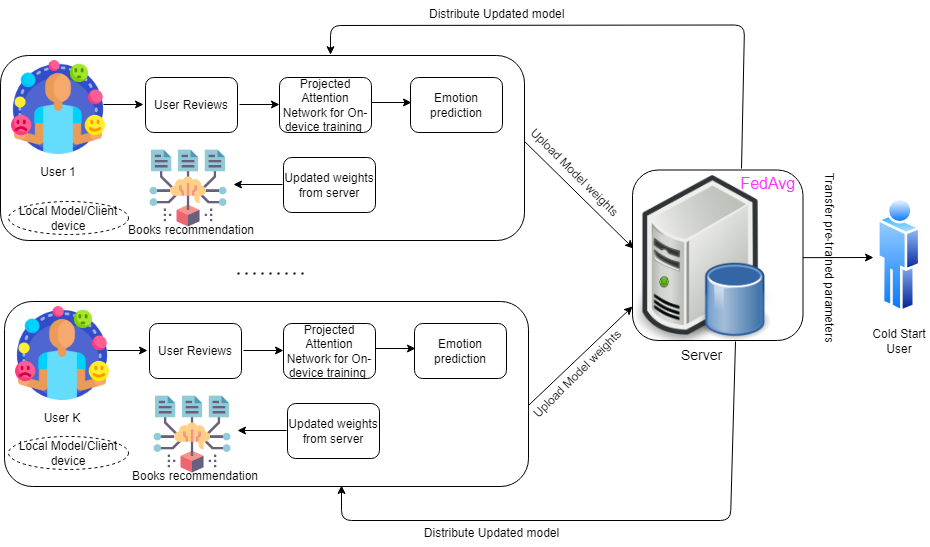
\includegraphics[width=0.8\textwidth]{figures/image23}
  \caption{Architecture of a Modular Federated Cross-Domain Recommendation System based on PRADO}
  \label{fig:ch4_f1}
\end{figure}

To tackle these limitations, a hybrid strategy, Buffered FedAvg, is used for global model training \cite{ref80} . In this approach, the server does not immediately combine the model after receiving each client's update. Instead, it temporarily saves the updates in a buffer. Only when the buffer reaches a predetermined threshold, M, does aggregation take place. That is, the server updates the model only after receiving M client updates, as shown in the following equation.

\begin{equation}
  w_{\text{server}}^{t+1}(\text{aggr}_{p}) = \frac{1}{M} \sum_{i \in B_{t}} w_{i}^{t}, \quad |B_{t}| \geq M
  \label{eq:ch4_4_1}
\end{equation}

$\mathbf{w}_{\text{global}}^{t+1}$ --- Aggregated global model parameters at round $t+1$.

$\mathbf{w}_{k}^{t}$ --- Local model parameters from client $k$ at round $t$.

$B_{t}$ --- Set (buffer) of participating clients in round $t$.

$M$ --- Minimum number of client updates required for aggregation (threshold).

$\text{aggr}_{p}$ --- Aggregation policy (e.g., FedAvg, Buffered FedAvg)

Until this condition is met, the server continues to gather updates without starting the aggregation process.

\subsection{Recommendation Module}
Each client uses the aggregated changes that are sent by the server to improve its local recommendation system. The following function is used to calculate the recommendation score $s_{i,j,k}$ at client $k$ for a given user $i$ and book $j$:

\begin{equation}
  s_{i,j,k} = f_{k}(u_{i}, t_{j}, e_{\text{agg}}, \text{rec\_score}_{k})
  \label{eq:ch4_rec}
\end{equation}

\noindent In this expression, $f_{k}$ denotes the client's recommendation function.

$u_{i}$ is the variable for the user representation, $t_{j}$ is a depiction of the target item, $e_{\text{agg}}$ represents the aggregation of emotional data that was obtained from the server, while $\text{rec\_score}_{k}$ contains the client's local recommendation model's parameters.

\section{GoEmotions Dataset Description} \cite{ref77}

Google scientists developed the GoEmotions dataset of 58,000 comments from Reddit. These remarks were gathered from English-language subreddits and carefully selected for psychological relevance and potential data uses. The dataset classifies emotions into 27 specific labels, plus a neutral category. Emojis serve as substitutes for emotional expression within the dataset. Table 4.3 shows an example comment with its associated emotional labels.

\begin{longtable}{|p{7cm}|p{7cm}|}
\caption{Samples from the GoEmotions dataset}
\label{tab:ch4_t1} \\
\hline
Reviews & Emotion label \\
\hline
\endfirsthead
\hline
Reviews & Emotion label \\
\hline
\endhead
\hline
\endfoot
I don't know but \ldots\ would be better \ldots. & Neutral \\
\hline
Thank you, kind stranger & Gratitude \\
\hline
I want a pizza flair!! & Desire \\
\hline
Still better than YouTube rewind\ldots & Admiration \\
\hline
Shhh don't give the idea & Anger \\
\hline
\end{longtable}

Figure 4.2 shows a horizontal bar plot illustrating the frequency distribution of emotions in the dataset. Each bar represents a specific emotion, with its length indicating how often it appears.

\begin{figure}[htbp]
  \centering
  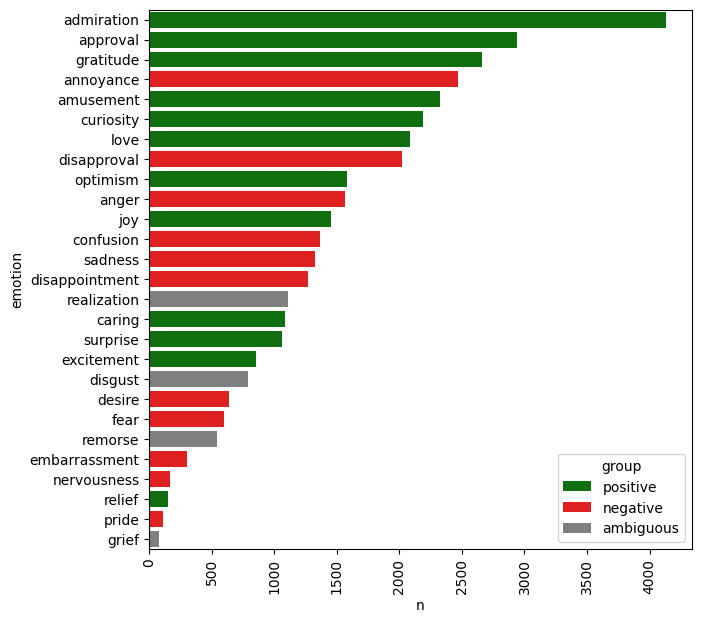
\includegraphics[width=0.8\textwidth]{figures/image24}
  \caption{Emotion distribution \cite{ref77}}
  \label{fig:ch4_f2}
\end{figure}

\section{Federated Framework Implementation}
This section describes how PRADO is used to build a federated learning framework that improves recommendation performance across domains (Emotions $\rightarrow$ Books, Emotions $\rightarrow$ Movies, Emotions $\rightarrow$ Songs, Emotions $\rightarrow$ Games). Despite the limited resources on client devices, PRADO manages on-device training efficiently. Identifying semantically similar terms is vital in this study, as it enhances recommendations across source and target domains. The trainable projection Model effectively captures long-range word dependencies and is proficient at categorizing lengthy texts.

All experiments in this research work are run on an Apple M4 Max (128 GB unified memory), GPU via Metal (tensorflow-metal 1.1.0), Python 3.11 with TensorFlow 2.15.1/Keras 2 and scikit-learn 1.9. Every notebook executes top-to-bottom under papermill on the seq-flow-lite-metal kernel. The aggregation server (MLServer; Spring Boot/Kotlin) runs on http://localhost:8080 and exposes setParamSeqFlow, getParamAvgSeqFlow, resetFedAvg, and fedAvgStatus with an aggregation buffer of 120. Section 4.5.1 provides an overview and notations used during implementation. Section 4.5.2 \& 4.5.3 elaborate federated training on the emotion model and the server aggregation process in depth, and Section 4.5.4 discusses the federated recommendation process.

\subsection{Overview and Notations}
The system studies content-based recommendation in which the only learned component is a federated text model. Two federated emotion models are trained on GoEmotions with K = 120

simulated clients: a fully federated PRADO network and a federated classification head on a frozen Small-BERT encoder \cite{ref98}. Aggregation is performed server-side by a Spring Boot service (MLServer) implementing streaming, buffered/weighted FedAvg (4.5.3).

Each target item $t_{i}$ (a movie, song, game, or book) is represented by a set of short text chunks $C_{i} = \{c_{1}, c_{2}, \ldots, c_{|C_{i}|}\}$ (plot sentences, four-line lyric stanzas, store-page sentences, or reviews). The end-to-end pipeline for one target item is:

\begin{equation}
  t_{i} \xrightarrow{\text{chunk}} C_{i} \xrightarrow{\text{fingerprint}} \{\phi(c) : c \in C_{i}\} \xrightarrow{\text{profile}} P_{i} \xrightarrow{\text{rank}} \text{score}(q, t_{i})
  \label{eq:ch4_pipeline}
\end{equation}

\noindent In this pipeline flow,

\begin{itemize}
    \item $t_{i}$ represents one target item: a movie, song, game, or book that can be recommended.
    \item $C_{i}$ represents the set of short text chunks describing the item: plot sentences, four-line lyric stanzas, store-page sentences, or reviews.
    \item $|C_{i}|$ is the number of chunks the item has.
    \item $c$ represents a single chunk (one short text) drawn from $C_{i}$.
    \item $\phi(c)$ represents the emotion fingerprint of chunk $c$: 27 numbers in $\mathbb{R}^{27}$, one per GoEmotions emotion (neutral is dropped), produced by a federated global model (Sec. 4).
    \item $e(c)$ represents the penultimate embedding: the federated PRADO model's 128-dimensional internal activation immediately before its output layer (Sec. 6). The 28 emotion scores are one linear function of $e(c)$, so $e(c)$ carries strictly more information than $\phi(c)$.
    \item $\mathbb{R}^{27}$ is the set of real-valued vectors with 27 components; writing $\phi(c) \in \mathbb{R}^{27}$ says that a fingerprint is a list of 27 real numbers.
    \item $|C_{i}|$ denotes target size and $\text{rank}(q)$ the rank of the query $q$'s target item under a given scorer.
\end{itemize}

denotes target size and  the rank of the query ’s target item under a given scorer.
In simple words, the end-to-end pipeline indicates that every item is broken into short texts; the federated model maps each short text to either a 27-emotion profile or a 128-number internal embedding; those vectors are then combined to represent, query, and rank items.

\subsection{Federated training of the emotion models}
Model training in the FL environment occurs on the local device with the distributed data, as mentioned in Section 3.3. The algorithm 1 demonstrates the key steps followed for training the model on the client-side using PRADO.

\begin{algorithm}[htbp]
\caption{Federated PRADO training (multi-round FedAvg). Takes the GoEmotions dataset as input. Data is divided among 120 clients. The model is trained for 20 communication rounds. During each round, 20 local training steps (epochs) are performed, with a batch size of 256, a learning rate of 0.5, and a momentum of 0.9. The weights are initialized to 5. The learning rate is scheduled using cosine decay (Eq.~\ref{eq:ch4_4_5}). Each client performs training on its own data using mini-batches. The weight $W$ at round $r$, $W_r$, at each internal training round is reset to zero to ensure every communication round starts with the same optimization settings. It updates the model parameters and minimizes the weighted binary cross-entropy loss (Eq.~\ref{eq:ch4_4_3}). The update process includes optimization using SGD (Eq.~\ref{eq:ch4_4_4}). After local training, the updated client models are sent back to the server, where they are aggregated using weighted Federated Averaging (Eq.~\ref{eq:ch4_4_6}) based on the number of local training samples. The aggregated model becomes the new global model and is redistributed for the next communication round. This iterative process continues until all communication rounds are completed, resulting in the final global PRADO model while preserving data privacy by keeping the training data on client devices.}
\label{alg:ch4_alg1}
\begin{algorithmic}[1]
\Require GoEmotions training set $\mathcal{D}$ (43,410 examples); clients $K=120$; rounds $R=20$; local steps $T=20$; batch $B=256$; peak rate $\eta=0.5$; momentum $0.9$; weight $w_d=5$
\Ensure global weights $W^*_R$; the final round's $K$ client models
\State Partition $\mathcal{D}$ into $K$ iid shards $\mathcal{D}_1,\ldots,\mathcal{D}_K$ by a seeded permutation (seed 42); persist the split
\State $W_0 \leftarrow$ a single shared random initialisation
\For{$r=0,\ldots,R-1$}
    \State $\eta_r \leftarrow \frac{\eta}{2}(1+\cos\frac{r\pi}{R})$ \hfill // cosine decay of Eq.~\ref{eq:ch4_4_5}
    \For{$k=1,\ldots,K$}
        \State \textbf{repeat}
        \State \quad load $W_r$; reset all optimiser state
        \State \quad run $T$ steps of the update of Eq.~\ref{eq:ch4_4_4} on $\mathcal{D}_k$, minimising Eq.~\ref{eq:ch4_4_3}
        \State \quad $W_{r,k} \leftarrow$ resulting weights; $m_{r,k} \leftarrow |\mathcal{D}_k|$
        \State \textbf{until} convergence
    \EndFor
    \State $W_{r+1} \leftarrow$ Eq.~\ref{eq:ch4_4_6}
\EndFor
\State persist $W^*_R$ as the client checkpoints uploaded in Algorithm~\ref{alg:ch4_alg2}
\end{algorithmic}
\end{algorithm}

\subsubsection{Model Output}
For an input text, the PRADO network produces one logit  per GoEmotions label, converted to an independent probability by the logistic sigmoid using equation (4.2):

\begin{equation}
  p_{l} = \sigma(z_{l}) = \frac{1}{1 + e^{-z_{l}}}, \quad l = 1, \ldots, 28
  \label{eq:ch4_4_2}
\end{equation}

$l$ --- the label index; GoEmotions has 28 emotion labels (27 emotions plus neutral).

$z_{l}$ --- the raw, unbounded score (logit) the network’s last linear layer assigns to label $l$.

$\sigma(\cdot)$ --- the logistic sigmoid function; it squashes any real number into the interval $[0,1]$.

$p_{l}$ --- the model’s predicted probability that the text expresses emotion $l$.

In simple words, equation (4.2) indicates each emotion gets its own independent yes/no probability. A sigmoid per label (rather than a softmax across labels) is what makes the problem multilabel: a text may be both “joy” and “surprise” at once, so the 28 probabilities need not sum to one.

\subsubsection{Minimize Client Loss}
The input dataset for PRADO is GoEmotions. The distribution of emotion frequency in dataset is shown in Figure 4.3. It indicates that there is majorable difference in number of samples of every emotiion. This affect on client’s performance. To minimize client loss, a positive-class--weighted binary cross-entropy (BCE) over the 28 labels is applied using equation (4.3):

\begin{equation}
  \mathcal{L}(y, p) = -\frac{1}{28} \sum_{l=1}^{28} \left[ w_{+} y_{l} \log p_{l} + (1 - y_{l}) \log(1 - p_{l}) \right], \quad w_{+} = 5
  \label{eq:ch4_4_3}
\end{equation}

$\mathcal{L}$ --- the loss (training penalty); smaller is better; training adjusts weights to reduce it.

$\mathbf{y}$ --- the ground-truth label vector; $y_{l} \in \{0, 1\}$ indicates whether emotion $l$ is truly present ($1$) or absent ($0$) in the example.

$\mathbf{p}$ --- the predicted probabilities from Eq. (4.2).

$\log(\cdot)$ --- the natural logarithm; $-\log(p)$ grows without bound as $p \to 0$, so confident mistakes are punished heavily.

$w_{+}$ --- the positive-class weight: the penalty for missing a present emotion is multiplied by 5.

$\frac{1}{28}$ --- the average over all 28 labels, so the loss scale does not depend on the label count.

For each label, the model pays a penalty  if the emotion is present (large penalty for assigning it low probability) and  if it is absent (large penalty for assigning it high probability); finally, the 28 penalties are averaged. The penalty applied (  ) is an essential component of more than just adjustment. As most emotion labels in the GOEmotions dataset occur infrequently, training with equal class weights (w sub plus equals 1) causes the model to favor predicting the absence of that emotion. In such cases, the large number of negative samples dominates the loss function, and the model achieves low recall for minority emotion classes. The penalty applied helps the model learn minority emotions more effectively. This results in balanced precision and recall.

\subsubsection{Optimization at Local Device}
During the first stage of experimentation, the Adam optimizer was used to optimize the client’s performance. However, it showed that this optimizer creates client-specific updates that prevented successful aggregation in federated learning. This prevents the global model from learning meaningful representations. Hence, in updated experimentation, each client runs Stochastic gradient descent (SGD) with momentum on its shard as given in equation (4.4).

\begin{equation}
  v \leftarrow 0.9v - \eta_{r} \nabla_{W} \mathcal{L}_{\mathcal{B}}(W), \quad W \leftarrow W + v
  \label{eq:ch4_4_4}
\end{equation}

$W$ --- the client’s current model weights (all trainable parameters, treated as one long vector).

$\nabla_{W} \mathcal{L}_{\mathcal{B}}(W)$ --- the gradient of the loss of Eq. (4.3), averaged over one mini-batch $\mathcal{B}$ ($|\mathcal{B}| = 256$).

$v$ --- the momentum (velocity) buffer, initialized to zero at the start of every round; it accumulates an exponentially decaying average of past gradients.

$0.9$ --- the momentum coefficient: 90\% of the previous velocity is retained each step, smoothing the descent direction.

$\eta_{r}$ --- the learning rate in round $r$ (Eq. (4.5) below): the step size.

The experimental footprints of the revised optimizer are discussed below.

\subsubsection{Scheduling Learning rate}
At early rounds of model training, the model requires large steps to make fast progress, and later it takes tiny steps. So the 120 clients stay close to the shared starting point and average cleanly. For a particular round, all clients use the same.  .  The learning rate is decayed across communication rounds by a cosine schedule.

\begin{equation}
  \eta_{r} = \frac{1}{2} \eta \left(1 + \cos \frac{\pi r}{R-1}\right), \quad r = 0, \ldots, R-1, \quad \eta = 0.5
  \label{eq:ch4_4_5}
\end{equation}

$\eta$ --- the peak learning rate, used in the first round.

$r$ --- the round index, running from $0$ to $R-1$.

$R$ --- the total number of communication rounds.

$\cos\frac{\pi r}{R-1}$ --- moves smoothly from $1$ (first round) to $-1$ (last round), so $\eta_{r}$ moves smoothly from $\eta$ down to $0$.

\subsubsection{Updated Server Aggregation}
The aggregation process demonstrated in equation (4.1) is updated as per the implementation requirement of the proposed model. The global model is updated using a weighted average (FedAvg) of the client models.

\begin{equation}
  W_{r+1} = \sum_{k=1}^{K} \frac{n_{k}}{n} W_{r}^{k}, \quad n = \sum_{k=1}^{K} n_{k}
  \label{eq:ch4_4_6}
\end{equation}

$K$ --- the number of clients: simulated parties, each holding a private data shard that never leaves it.

$W_{r}^{k}$ --- client $k$’s weights after its local training in round $r$ (each client started the round from the same global $W_{r}$).

$n_{k}$ --- the number of training examples on client $k$ (here 361--362).

$n$ --- the total number of examples across all clients (43,410).

$\frac{n_{k}}{n}$ --- client $k$’s mixing weight: clients with more data count proportionally more. The weights sum to 1, so the result is a convex combination.

$W_{r+1}$ --- the new global model broadcast at the start of the next round.

As demonstrated in the last step of Algorithm 1, the client’s weights are uploaded to the server. They are further processed according to the Server-side aggregation protocol.

\subsection{Server-side aggregation protocol}
MLServer (server-Spring Boot service) maintains a running weighted sum $S$, a sample total $n$, an upload counter $c$, and the last computed average $A$. Uploads are JSON weight sets with the client’s shard size. On each upload $(w, n_k)$ the server performs the streaming update

\begin{equation}
  S \leftarrow S + n_{k} \cdot \text{flatten}(w), \quad n \leftarrow n + n_{k}, \quad c \leftarrow c + 1
  \label{eq:ch4_4_7}
\end{equation}

$w$ --- one client’s uploaded weights (a structured set of arrays).

$\text{flatten}(w)$ --- those arrays concatenated into one long vector, so the server does arithmetic on a single vector regardless of the model’s layer structure.

$S$ --- the running weighted sum of all flattened uploads so far. Only this one vector is stored --- never the 120 individual uploads.

$n$ --- the running total of shard sizes; $c$ --- how many clients have uploaded in the current round.  Equation (4.7) indicates that each upload is folded into a single accumulator vector and then discarded. Memory cost is of only one model, not 120. When the counter reaches the buffer size ($c = 120$) the average is computed asynchronously, in a background coroutine:

\begin{equation}
  A \leftarrow \text{unflatten}(S/n), \quad S \leftarrow n \cdot \text{flatten}(A), \quad c \leftarrow 0
  \label{eq:ch4_4_8}
\end{equation}

$A$ --- the sample-weighted mean of Eq. (4.6), computed in flattened form; restores the original layer structure.

$A$ --- the last computed global average, served by GET /getParamAvg (HTTP 409 ``Conflict'' if none exists yet).

$c$ --- re-seeding: the accumulator is reset to "$S \leftarrow n \cdot \text{flatten}(A)$", weighted by all $n$ samples seen, so the next round's uploads blend with the current global model rather than starting from zero.

Averaging runs as a coroutine; the 120th upload’s HTTP response returns before the average exists. Clients must poll /fedAvgStatus until $c$ has returned to $0$ before fetching $A$, or risk reading a stale result of HTTP 409. The complete process is described stepwise in Algorithm2.

In Algorithm 2, $m$ represents the method an endpoint refers to: $w$ seqFlowLite (PRADO), $W$ represents the fetched global weights; $S$ represents the running sum; validation (line 1) represents that every upload’s array shapes, element types, and finiteness (no NaN/Inf) are checked against the round’s first upload, so one malformed client cannot silently corrupt $W_r$.

\begin{algorithm}[htbp]
\caption{Streaming weighted FedAvg on MLServer, and the client protocol. All locally trained model parameters, uploaded by clients, are first validated by the server to ensure consistency. The next step performs a streaming update (Eq.~\ref{eq:ch4_4_9}), i.e., received model weights are added to the aggregation buffer. This process continues until updates for all clients are received. Once updates from all clients are received, the buffered FedAvg is performed to generate new global weights.}
\label{alg:ch4_alg2}
\begin{algorithmic}[1]
\State \textbf{Server, on} \texttt{POST /setParam($m$)} with $(w, n_x)$:
\State \quad validate leaf types, finiteness, and weight count against the round's first client
\State \quad apply the streaming update of Eq.~\ref{eq:ch4_4_9}
\If{$c = 120$} \hfill // asynchronously, in a coroutine
\State \quad apply the averaging step of Eq.~\ref{eq:ch4_4_10} \hfill // $A$ seeds the next round
\EndIf
\State \textbf{Server, on} \texttt{POST /resetFedAvg}: $S, n, c \leftarrow 0$ ($A$ remains readable)
\State \textbf{Server, on} \texttt{GET /getParamAvg($m$)}: return $A$ (HTTP 409 if absent)
\State \textbf{Client upload procedure} (\texttt{ensure\_global\_weights}):
\If{GET /getParamAvg succeeds}
\State \quad use $A$ (fast path)
\Else
\State \quad \texttt{POST /resetFedAvg}; upload the 120 checkpoints with shard sizes
\State \quad poll \texttt{/fedAvgStatus} until $c = 0$ \hfill // averaging is asynchronous
\State \quad $W_{\text{glob}} \leftarrow$ GET \texttt{/getParamAvg}
\EndIf
\end{algorithmic}
\end{algorithm}

The third part of this process includes fingerprint extraction with a federated global model given in Algorithm 3.

\begin{algorithm}[htbp]
\caption{Fingerprint extraction with a federated global model. The emotion fingerprint is a fixed-length vector containing the predicted probabilities of all emotion classes (excluding the neutral class). It is a compact emotional representation of a text and is used for subsequent recommendation and similarity computations.}
\label{alg:ch4_alg3}
\begin{algorithmic}[1]
\Require text $t$; federated global model (PRADO or BERT head) from Algorithm~\ref{alg:ch4_alg2}
\State normalise whitespace in $t$
\If{model is PRADO FL}
\State $p \leftarrow \text{PRADO}_{\text{FedAvg}}(t)$ \hfill // raw string in; 28 sigmoid scores out
\Else
\State ids $\leftarrow$ WordPiece($t$), length 40; $x \leftarrow$ masked mean (Eq.~\ref{eq:ch4_4_7})
\State $p \leftarrow \text{head}_{\text{FedAvg}}(x)$
\EndIf
\Return $\phi(t) = p_{1:27}$ \hfill // label 28, neutral, is dropped
\end{algorithmic}
\end{algorithm}

\begin{equation}
  \phi(t) = (p_{1}, \ldots, p_{27}) = p_{1:27}, \quad p = \begin{cases} \text{PRADO}_{\text{FedAvg}}(t) & (\text{PRADO path}) \\ \text{head}_{\text{FedAvg}}(x_{t}) & (\text{BERT path}) \end{cases}
  \label{eq:ch4_4_9}
\end{equation}

--- the federated PRADO model applied to the raw string  (PRADO tokenizes internally); output is the 28 sigmoid scores of Eq. (4.2),  --- the first 27 of the 28 scores: label 28, neutral, is dropped.

\subsection{Federated Recommendation Process}
In sections 4.5.2 \& 4.5.3, a detailed discussion of federated emotion extraction and its server aggregation process is given. The recommendation process is implemented and assessed across three methods: the first using a Random Forest classifier, the second using 28-emotion probable output from PRADO (Featured Recommender Version1-V1), and the third using the model’s 128-dimensional penultimate representation (Featured Recommender Version2-V2). These implementations also provide their contribution to the final performance of the proposed model.

\subsubsection{Random-forest fingerprint lookup}
In case a random forest classifier is used in the original form, with a fixed decision tree, random-threshold splits, and no bootstrapping, its behavior is explained here. The input of the classifier is the emotion fingerprint of a review, and the output is the name of the book that this review belongs to. The model is trained on 10,000 sampled reviews, which correspond to 9,970 different book titles, so that almost all titles have only one book review. In recommendation, the model calculates the probability scores returned by predict\_proba($\phi(t)$) for candidate books and recommends the top-n books. The model simulates the original notebook's high accuracy of 99.54\% when performing the evaluation task in the original notebook's style using the proposed federated emotion fingerprints.

However, this high accuracy does not indicate that the recommender generalizes well to unseen data. Its performance is fundamentally limited by the following structural ceiling:

\begin{equation}
  \text{ceiling} = \frac{\left| \{ q \in D_{\text{test}} : \text{title}(q) \in \mathcal{Y}_{\text{train}} \} \right|}{|D_{\text{test}}|} = 0.40\%
  \label{eq:ch4_4_10}
\end{equation}

• $D_{\text{test}}$ --- the held-out 20\% of reviews under an 80/20 split; $\text{title}(q)$ --- the true book title of a test review $q$.

• $Y_{\text{train}}$ --- the set of titles that appear in the training data, i.e. the classifier’s label space.

• ceiling --- the fraction of test queries whose correct answer the classifier is even able to output. No classifier of this design can exceed it.

In this dataset, almost all book titles are unique. Once the data is split, the review of a specific book will usually be in the training set or the test set but not both. As a result, the proportion of the test reviews that match a classifier's previous classification is 0.40\%. To be precise, for the remaining 99.60\% of test titles, no classifiers will be able to predict the label, even if the classifiers are well trained.

Thus, the held-out accuracy observed is just 0.20\%, about half of the theoretical (0.40\%) accuracy. This indicates that the Random Forest focuses on the mapping between an emotion fingerprint and a book title, not on learning patterns that apply to unknown books.

\subsubsection{Featured Recommender Version1 (v1)}
The emotion classification model produces a 27-dimensional emotion fingerprint for each text chunk. This section describes how to generate recommendations and evaluate them. The main objective is to recommend the correct target item (book, song, movie, game, etc.) based on its emotional characteristics rather than memorizing titles. Below is a step-by-step explanation.

\subsubsection{Step 1: Build an item’s emotional profile (Eq.4.11)}
The chunks may contain multiple views; the mean of all these chunks is calculated using equation (4.11) and mapped over 27 emotions.

\begin{equation}
  P_{i} = \frac{1}{|C_{i}|} \sum_{c \in C_{i}} \phi(c) \in \mathbb{R}^{27}
  \label{eq:ch4_4_11}
\end{equation}

• $P_i$ --- item $i$'s emotion profile: mean fingerprint of all its chunks.

• $\frac{1}{|C_i|} \sum_{c \in C_i}$ --- arithmetic mean over item's chunk set.

\subsubsection{Step 2: Standardisation of  each emotion dimension (Eq.4.12)}
The review text may have different emotions at different scales. For example, a sentence may contain emotions related to joy, gratitude, anger, and fear, with a higher average score for joy; if cosine similarity is computed directly, it may dominate the selection of the correct target item. To solve this problem, every emotion dimension is converted to z-score using Eq.(4.12)

\begin{equation}
  \begin{aligned}
  z(v)_{d} &= \frac{v_{d} - \mu_{d}}{\sigma_{d}}, \\
  \mu_{d} &= \frac{1}{N} \sum_{i=1}^{N} (P_{i})_{d}, \\
  \sigma_{d}^{2} &= \frac{1}{N} \sum_{i=1}^{N} \left( (P_{i})_{d} - \mu_{d} \right)^{2}
  \end{aligned}
  \label{eq:ch4_4_12}
\end{equation}

• $v_d$ --- the $d$-th component ($d=1,\ldots,27$) of fingerprint vector $v$.

• $\mu_d$, $\sigma_d$ --- mean and std. of dimension $d$ over all $N$ target item profiles.

• $z(v)$ --- the standardized vector: every dimension now has zero mean and unit variance across the target items.

Step 3: Compare the item’s standardized emotional profile with the user query Eq. 4.13)

\subsubsection{Step 3: Compare the item's standardized emotional profile with the user query (Eq. 4.13)}
The standardized emotional profile is compared with the user query using Equation (4.13). Items are ranked by cosine similarity of the standardized vectors. Cosine similarity itself is

\begin{equation}
  \cos(a, b) = \frac{a \cdot b}{\|a\| \, \|b\|} = \frac{\sum_{d} a_{d} b_{d}}{\sqrt{\sum_{d} a_{d}^{2}} \, \sqrt{\sum_{d} b_{d}^{2}}} \in [-1, 1]
  \label{eq:ch4_4_13}
\end{equation}

• $a \cdot b$ --- the dot product of the two vectors; $\|a\|$ --- the Euclidean length of $a$.

• $\cos(a, b)$ --- the cosine of the angle between $a$ and $b$: $1$ for identical directions, $0$ for unrelated (orthogonal) ones, $-1$ for opposite ones. It ignores vector magnitude entirely, and the v1 ranking score is

Each emotion profile is an arrow in a 27-dimensional vector. Cosine similarity measures the angle between the two arrows. It returns 1 if the emotional patterns are the same or 0 if the emotional patterns are opposite.

\subsubsection{Step 4: Recommendation score computation (Eq. 4.14)}
The recommendation score is computed using Eq. 4.12 and 4.13. Eq. (4.14) shows the combined version for computing it.

\begin{equation}
  s(q, i) = \cos\left( z(\phi(q)), \, z(P_{i}) \right)
  \label{eq:ch4_4_14}
\end{equation}

• $q$ --- the query: a single held-out chunk; $\phi(q)$ emotions fingerprint (Eq. (4.11)).

• $z(\cdot)$ --- the target item's standardization of Eq. (4.12), applied to both sides.

• $s(q, i)$ --- the score by which all $N$ items are sorted (descending) to produce the recommendation list for $q$.

Duplicate-chunk guardrail.

In all corpora, duplicate chunks (after normalizing text) are eliminated within the items. This is not a preference, but a correctness requirement: Amazon presents the same review text as multiple review editions (37\% of the number of rows in the multi-review table), and song choruses repeat ($\sim$6\% of the number of rows in the table of stanzas); with duplicates in place, held-out ``retrieval'' becomes duplicate matching, and the median rank is 1 (before fix).

\subsubsection{Hold-one-out evaluation}
For each $|C_i| \ge 2$, one chunk is held out (seed 42): all profiles are rebuilt without the held-out chunks; each held-out chunk queries the whole catalog: the rank of its own item feeds the metrics of Sec. 7 (at most 3,000 queries). The difficulty in rebuilding the profiles without the chunk shown makes evaluation fair: the query text doesn't ''push'' into the profile it's trying to build.

\subsubsection{Featured recommender Version2(v2)}
The second version of the recommendation system(V2) is discussed in this section. This system does not retrain the Federated PRADO. It uses the model weights from Section 4.5.2. It combines three complementary similarity views to capture different information about the target item. The following three changes convert the same federated PRADO model into a substantially stronger retriever. (i) Instead of probable emotion, retrieval uses the model’s 128-dimensional penultimate representation  (the concatenated attention-pooled bigram and trigram channels). The emotion scores are a single linear readout:  with . Working with  retains everything the federation learned about the text, not only its projection onto 28 emotions.

(ii) Document queries. For every item with , a random half  forms the query document and the complement  the profile. The split precedes any windowing, so no text occurs on both sides; the ranked target item is always the full one.

(iii) Ensemble scorer. Embedding centroids are first PCA whitened. The whitening transformation first centres the data, then rotates it into principal directions and then scales every direction to unit variance. Equation (4.15) gives the whitening transform, fitted on the  profile centroids (respectively on a 60k-chunk sample for ), is

\begin{equation}
  \begin{aligned}
  \Psi(x) &= \text{diag}\!\left( \frac{s_{j}}{\sqrt{n-1}} + \varepsilon \right)^{-1} V^{\top}(x - \mu) \\
  \widetilde{X} &= X - \mathbf{1}\mu^{\top} = U \, \text{diag}(s) \, V^{\top}
  \end{aligned}
  \label{eq:ch4_4_15}
\end{equation}

• $X$ --- the matrix whose rows are the fitting vectors (profile centroids, or the 60k chunk embeddings); $n$ --- the number of rows; $\mu$ --- their mean vector, subtracted from every row.

• $X = U \, \text{diag}(s) \, V^\top$ --- the singular value decomposition of the centred matrix: $V$'s columns are the principal directions (axes of greatest variance), and the singular values $s_j$ measure the data's spread along each.

• $V^\top(x - \mu)$ --- centre the input and rotate it into the principal-axis coordinate system.

• $\text{diag}(s_j / \sqrt{n-1} + \varepsilon)^{-1}$ --- divide each rotated coordinate by that axis's standard deviation, so every axis has unit variance after the transform.

• $\varepsilon = 10^{-6}$ --- a numerical floor preventing division by near-zero singular values on nearly flat directions.

• $\Psi(x)$ --- the whitened vector.

Whitening makes cosine similarity focus on meaningful differences instead of common characteristics like writing style, sentence length, common vocabulary, etc. (for books as the target item). If cosine similarity is applied directly/ then the common characteristics create bias in recommendation. The extension of three changes is described as 3 views.

View 1: Centroid Cosine(whitened):- chunk embeddings from each document half are averaged into one vector. E.g. chunk1,chunk2,chunk3  Average  Centroid. The cosine similarity between the query and candidate centroid is computed. It captures the general topic of the document.

\begin{equation}
  \begin{aligned}
  S_{1}(q, i) &= \cos\!\left( \Psi\!\left( \overline{e}(Q_{q}) \right), \, \Psi\!\left( \overline{e}(P_{i}) \right) \right) \\
  \overline{e}(X) &= \frac{1}{|X|} \sum_{c \in X} e(c)
  \end{aligned}
  \label{eq:ch4_4_16}
\end{equation}

• $Q_q$ --- the query half of the querying item's chunks; $P_i$ --- the profile half of the candidate item $i$'s chunks.

• $\overline{e}(X)$ --- the centroid: the mean of the embeddings of the chunk set $X$; one 128-dimensional summary vector per side.

• $S_1(q, i)$ --- whitened-centroid cosine: how similar the query document's average embedding is to the candidate's average embedding.

View 2: It repeats view1 for neighboring sentences, i.e., a 2-chunk window. It helps to capture the relationship among neighboring sentences, context, and narrative flow, given by Eq.(4.17)

\begin{equation}
  S_{2}(q, i) = S_{1}, \text{ but with } e(\cdot) \text{ applied to 2-chunk windows formed inside each half}
  \label{eq:ch4_4_17}
\end{equation}

• 2-chunk window --- two consecutive chunks of one half concatenated and embedded as a single text, giving the model slightly longer context than a lone sentence or stanza.

• “inside each half” --- windows never span the query/profile boundary, preserving the leak-free split of design choice (ii).

View 3: It is a late interaction score: there is no pooling of summaries; each query sentence searches the candidate for the matching sentence. It rewards items that match specific sentences rather than the overall blend, complementing the centroid views given by Eq.(4.17)

\begin{equation}
  S_{3}(q, i) = \frac{1}{|Q_{q}|} \sum_{c \in Q_{q}} \max_{c' \in P_{i}} \cos\left( \Psi(e(c)), \, \Psi(e(c')) \right)
  \label{eq:ch4_4_18}
\end{equation}

• $c$ --- one individual query chunk; $c'$ --- one individual profile chunk of the candidate $i$.

• $\max_{c' \in P_i}$ --- each query chunk's similarity to its single best-matching profile chunk of the candidate.

• $\frac{1}{|Q_q|} \sum_{c \in Q_q}$ --- the query's chunks then vote by averaging their best-match scores.

\subsubsection{Standardizing the view scores}
These similarity views produce scores on different scales, like 0.91, 15, or 0.25. Hence, before fusing, each view’s score row is standardized per query using Eq.(4.18)

\begin{equation}
  \zeta(S)_{q,i} = \frac{S(q, i) - \text{mean}_{i'} \, S(q, i')}{\text{std}_{i'} \, S(q, i')}
  \label{eq:ch4_4_18_dup}
\end{equation}

• $\text{mean}_{i'}$, $\text{std}_{i'$} --- mean and standard deviation taken over all $N$ candidate items for the same query $q$ (i.e. across one row of the score matrix).

• $\zeta(S)_{q,i}$ --- item $i$'s score re-expressed The final ensemble score is the weighted sum

\begin{equation}
  S(q, \cdot) = w_{1} \, \zeta(S_{1}) + w_{2} \, \zeta(S_{2}) + w_{3} \, \zeta(S_{3})
  \label{eq:ch4_4_19}
\end{equation}

• $w_1, w_2, w_3$ --- non-negative per-domain fusion weights, tuned on a seed-42 grid: movies $(0.3/0.2/0.5)$, music $(0.4/0.0/0.6)$, games $(0.25/0.15/0.6)$, books $(0.35/0.1/0.55)$.

• $S(q, \cdot)$ --- the fused score of every target item for the query $q$; items are ranked by it in descending order.

The v2 retrieval framework boosts recommendation accuracy without the need to retrain the federated model PRADO. Instead, it provides more enriched embeddings, a more leakage-free document-splitting strategy, PCA-based whitening, and a three-view ensemble ranking method using the learned representations. The 128-dimensional embeddings contain significantly more meaning than the final emotion probabilities, and the split-half evaluation guarantees unbiased evaluation. Whitening is used to remove uninformative embedding directions that dominate the embedding, and the ensemble consists of document-level summaries, contextual windows, and sentence-level matching, all with a combined ranking score. These enhancements can be used together to enable the recommender to retrieve items by deeper semantic and emotional similarity (meaning that they are not just remembered, but also understood), leading to a stronger and more generalizable recommendation system.

\begin{algorithm}[htbp]
\caption{PRADO FL v2: federated embeddings, split-half document queries, three-view ensemble.}
\label{alg:ch4_alg4}
\begin{algorithmic}[1]
\Require chunked catalogue $\{C_i\}$; federated PRADO weights (Algorithm~\ref{alg:ch4_alg2})
\State $e(c) \leftarrow$ penultimate PRADO activation for every chunk $c$
\State split each $C_i$ ($|C_i| \geq 4$) into query half $Q_i$ and profile half $P_i$ (seed 42), before any windowing
\State compute $S_1, S_2, S_3$ by Eqs.~\ref{eq:ch4_4_17}--\ref{eq:ch4_4_18} over the full catalogue
\State fuse by Eqs.~\ref{eq:ch4_4_19}--\ref{eq:ch4_4_19} with the domain's weights; rank items
\State evaluate with Sec.~7 (3,000 queries, seed 42)
\end{algorithmic}
\end{algorithm}

The complete process discussed in Section 4.5 is summarized in the following steps

\subsubsection{Pipeline (identical in every domain notebook):}
The FL global emotion model is fetched from MLServer (120-client weighted FedAvg; the saved client checkpoints are uploaded first if the server holds no average). PRADO consumes raw strings; BERT is the federated classifier head on top of the frozen Small BERT encoder (shared preprocessing).

Every item's text is split into GoEmotions-comment-sized chunks: plot sentences for Movies, review text for Books, 4-line lyric stanzas for Music, and store-page sentences for Games. Each chunk becomes a 27-dim emotion fingerprint (neutral dropped).

An item's emotional profile is the mean of its chunk fingerprints (multiple texts per item).

Recommender: Two versions of recommenders (V1 and V2) are implemented, using cosine similarity between z-scored profiles (z-scoring per emotion dimension across the catalog stops uniformly-loud dimensions from drowning rare, discriminative ones --- measured in the raw-vs-z ablation (Equations 4.15-4.19).

\subsubsection{Runtime details and reproducibility}
Uploading a full federated round takes 13 s (120 PRADO models) and 80 s (120 BERT heads); server averaging completes in seconds. Fingerprinting the largest corpus (movies, 255,602 chunks) takes 4 s with PRADO versus 297 s with BERT (68); the two v2 embedding views cost 6 s. Federated training itself takes 11 min (PRADO,  client fits) and 2 min (BERT heads); the recommendation suite reuses the persisted final-round checkpoints. All sampling, splits, and tuning grids derive from seed 42 and reproduce digit-for-digit; per-notebook JSON artifacts (metrics, ranks, timings) feed both companion documents, and a single shared module (fl\_common.py) implements every algorithm above.

\section{Performance Analysis}
This section outlines the performance analysis of the proposed advancements in basic Modular Federated CDR on emotion classification and cross-domain recommendation.

\subsection{Client Optimizer ablation (Equation 4.4)}
The revision of the training process is grounded in a controlled ablation over client optimizers and local-work budgets, run on identical shards from the identical initialization (fixed seed; every configuration is exactly reproducible). Adam clients --- the original choice --- leave the global model at chance level: their per-parameter adaptive scaling turns the 120 local updates into mutually incoherent directions whose average carries almost no signal. Replacing the client optimizer with SGD + momentum turns federated averaging constructive, and quality then scales with local work and learning rate: at lr 0.5 with 20 local steps the global model passes the best Adam variant within two rounds and reaches 0.20 test loss by round four. This single change explains the difference between the collapsed one-shot results and the revised process. The same mechanism, amplified by their dominant trainable embedding tables (2.56M of \textasciitilde{}2.7M parameters trained on \textasciitilde{}362 examples per client), is what destroys the one-shot federated LSTM and Bi-LSTM: each client's embedding rows co-adapt with its own recurrent gates, the 120 configurations are mutually incompatible, and their average passes no input signal --- the averaged network outputs each label's base rate for every input, hence deceptively low loss with zero precision and recall. BERT is insulated because its encoder is frozen and shared, leaving only a near-convex head to average.

\begin{figure}[htbp]
  \centering
  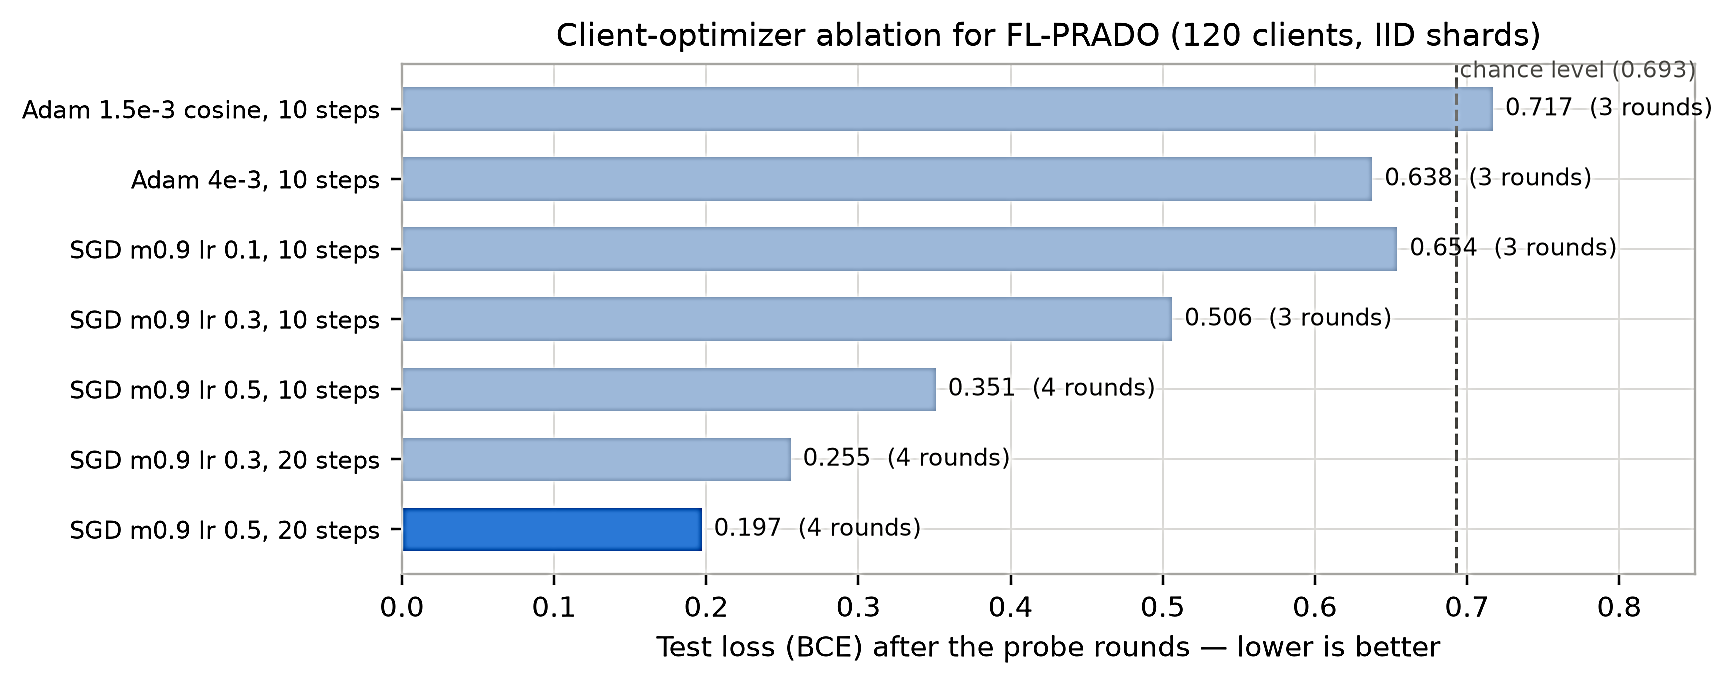
\includegraphics[width=0.8\textwidth]{figures/image29}
  \caption{Client-optimizer ablation: test loss of the FL-PRADO global model}
  \label{fig:ch4_f7}
\end{figure}

\subsection{Operating-Point Control: Positive-Class Weight}
\begin{longtable}{|c|c|c|c|c|}
\caption{Effect of positive weight class in client objective}
\label{tab:ch4_t2} \\
\hline
POS\_WEIGHT & Test Loss & Precision@5 & Recall@5 & F1-Score \\
\hline
\endfirsthead
\hline
POS\_WEIGHT & Test Loss & Precision@5 & Recall@5 & F1-Score \\
\hline
\endhead
\hline
\endfoot
1 & 0.157 & 0.724 & 0.098 & 0.172 \\
\hline
3 & 0.160 & 0.517 & 0.390 & 0.445 \\
\hline
5 & 0.174 & 0.469 & 0.477 & 0.473 \\
\hline
\end{longtable}

With the plain objective (weight 1) the federated model converges to an extremely conservative solution --- excellent precision but recall 0.10, and a threshold sweep shows its precision-recall curve cannot reach the centralized operating point at any threshold, so no post-hoc calibration can repair it. Weight 3 matches the centralized recall (0.39) at precision 0.52; weight 5 maximizes F1 at a balanced operating point and is the default of the revised process. Figure 4.6-K places the resulting model's full precision-recall trade-off next to the centralized PRADO operating point. The effect of positive weight class is listed in Table 4.6.1 and its graph is shown in Figure 4.6.2. Figure 4.6.3 shows the trade-off of the final FL-PRADO global model.

\clearpage
\begin{figure}[htbp]
  \centering
  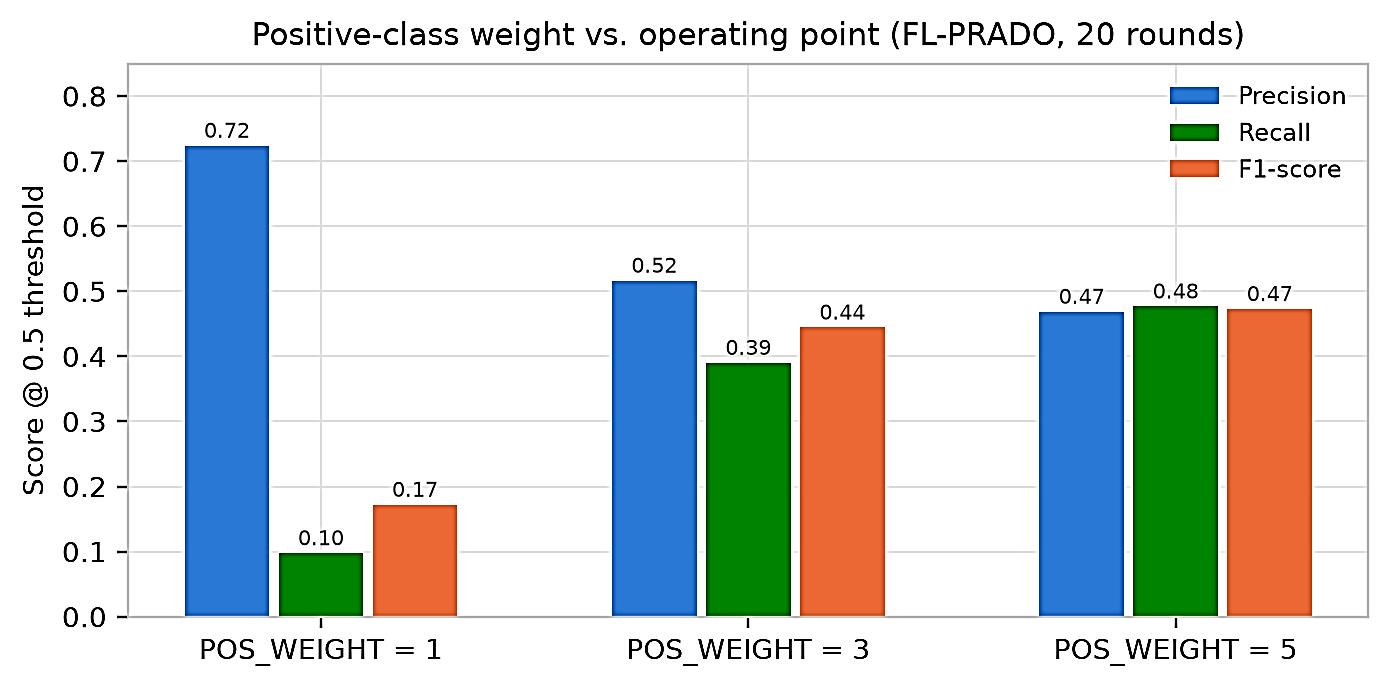
\includegraphics[width=0.8\textwidth]{figures/image30}
  \caption{Precision/recall/F1 at the 0.5 threshold as a function of the positive-class weight (FL-PRADO, 20 rounds)}
  \label{fig:ch4_f8}
\end{figure}

\begin{figure}[htbp]
  \centering
  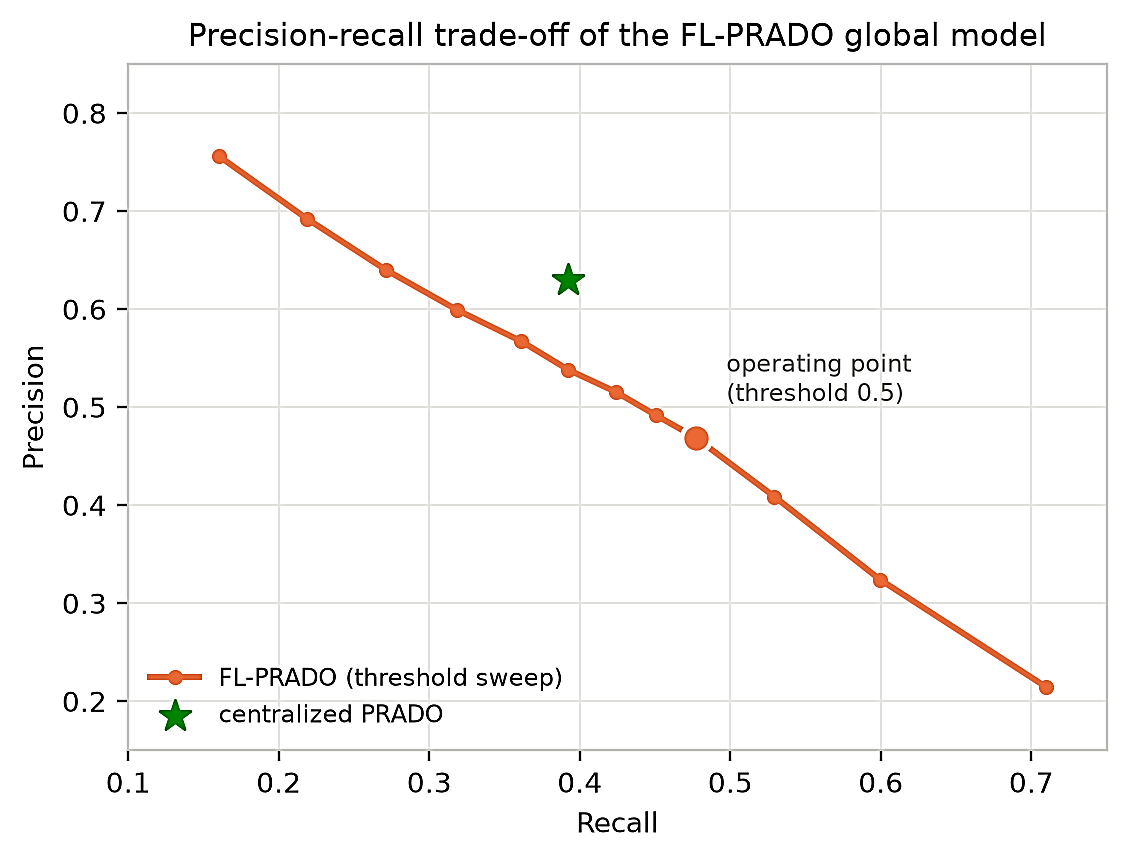
\includegraphics[width=0.8\textwidth]{figures/image31}
  \caption{Precision-recall trade-off of the final FL-PRADO global model}
  \label{fig:ch4_f9}
\end{figure}

The centralized PRADO reference point has higher precision and lower recall, and FL-PRADO has higher recall and acceptable precision. Overall, FL-PRADO is flexible, enabling a proper trade-off between prediction accuracy and coverage while maintaining the privacy of federated learning.

\subsection{Qualitative Results}
Table 4.3 presents the top-3 predicted emotions for the three reference prompts, generated by the federated PRADO model. The predictions from the local weighted-average model and the MLServer aggregation endpoint are nearly identical (matching to float32 precision). The revised federated PRADO reproduces the centralized top predictions with comparable confidence, and on ''I love you,'' its secondary predictions are arguably more sensible than the centralized model's spurious nervousness (0.989).

\begin{longtable}{|p{3cm}|p{3.5cm}|p{3.5cm}|p{3.5cm}|}
\caption{Comparative Confidence Score for Emotion Predictions across models}
\label{tab:ch4_t3} \\
\hline
\makecell{Input \\ text} & PRADO & \makecell{PRADO FL \\ (revised)} & \makecell{BERT FL \\ (one-shot)} \\
\hline
\endfirsthead
\hline
\makecell{Input \\ text} & PRADO & \makecell{PRADO FL \\ (revised)} & \makecell{BERT FL \\ (one-shot)} \\
\hline
\endhead
\hline
\endfoot
\makecell{``Good \\ for you!''} & \makecell{admiration 0.897 \\ caring 0.331 \\ approval 0.328} & \makecell{admiration 0.944 \\ caring 0.549 \\ gratitude 0.468} & \makecell{admiration 0.676 \\ gratitude 0.613 \\ caring 0.011} \\
\hline
\makecell{``Happy \\ birthday!''} & \makecell{joy 0.850 \\ excitement 0.722 \\ surprise 0.308} & \makecell{joy 0.975 \\ excitement 0.621 \\ neutral 0.243} & \makecell{admiration 0.181 \\ gratitude 0.102 \\ joy 0.063} \\
\hline
\makecell{``I love \\ you.'' } & \makecell{love 1.000 \\ nervousness 0.989 \\ amusement 0.350} & \makecell{love 0.998 \\ joy 0.250 \\ gratitude 0.208} & \makecell{love 0.973 \\ admiration 0.032 \\ caring 0.014} \\
\hline
\end{longtable}

\section{Summary}
This chapter introduced the Multi-Objective and Modular Federated Cross-Domain Recommendation (MFCDR) framework, combining PRADO, Weighted FedAvg, and a modular recommendation strategy for privacy-preserving cross-domain recommendation. The federated training framework, server-side aggregation protocol, and recommendation process were detailed. Two feature-based approaches (V1 and V2) assessed emotion-based representations for Books, Movies, Music, and Games. The framework's effectiveness was verified through optimizer ablation, operating point evaluation, and qualitative assessment. This accomplishes Objective~3.

